% Figure 1: Univariate Regressions
\begin{figure}[htbp]
\centering
\caption{Predictors of Post-Treatment Bilateral Connectivity: Univariate Regressions}

\begin{threeparttable}
\label{fig:bilateral_coefplot_univariate}

\begin{subfigure}{0.49\textwidth}
    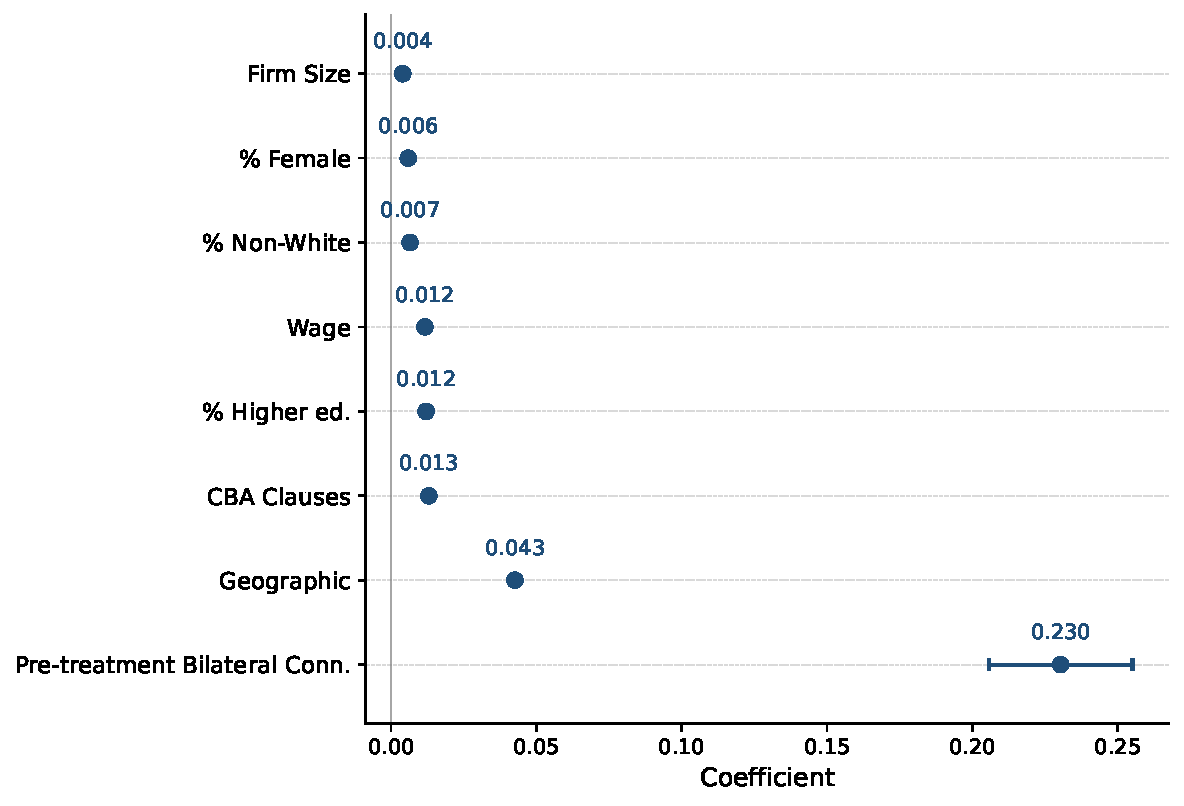
\includegraphics[width=\textwidth]{coefplot_bilateral_proximity_univariate.pdf}
    \caption{Proximity Measures}
    \label{fig:bilateral_proximity_univariate}
\end{subfigure}
\begin{subfigure}{0.49\textwidth}
    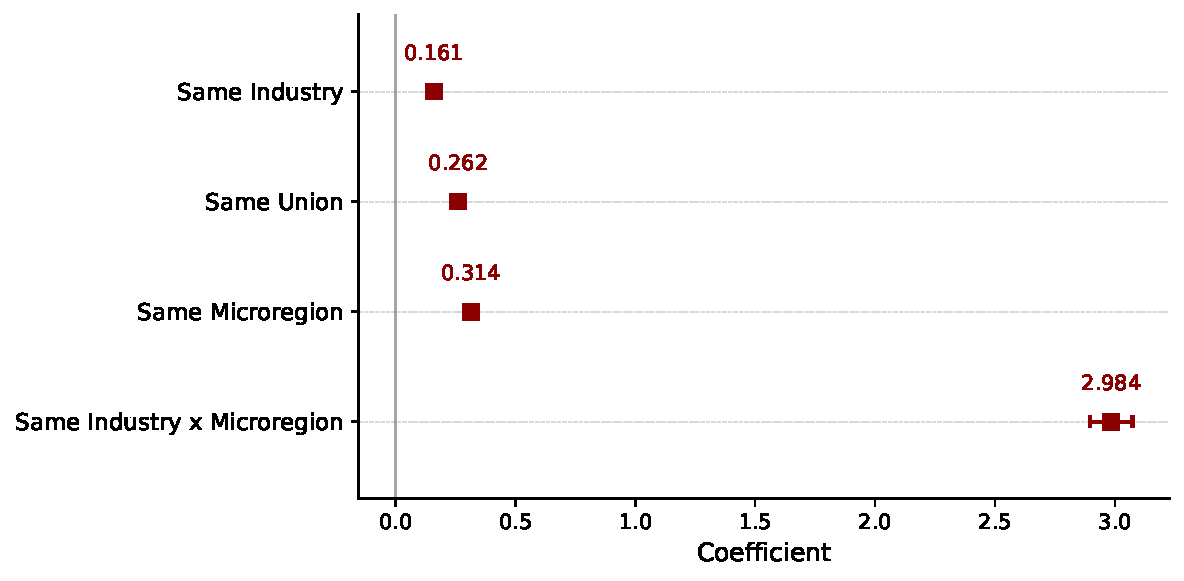
\includegraphics[width=\textwidth]{coefplot_bilateral_dummies_univariate.pdf}
    \caption{Same-Category Dummies}
    \label{fig:bilateral_dummies_univariate}
\end{subfigure}

\begin{tablenotes}
\footnotesize
\item \textit{Notes:} Each coefficient is from a separate regression of post-treatment bilateral connectivity (2011--2015) on the indicated predictor, controlling for establishment $i$ fixed effects. Bilateral connectivity is measured as the person-weighted average flow of workers between establishment pairs across four consecutive year-pairs. Proximity measures are defined as the negative absolute difference between establishment characteristics (standardized), so higher values indicate greater similarity. Geographic proximity is measured as the negative log of distance between municipality centroids. CBA clauses proximity is based on the number of clauses in collective bargaining agreements. Same-category dummies equal one if both establishments share the indicated category. Establishment characteristics are based on 2009--2011 pre-treatment averages. Horizontal lines represent 95\% confidence intervals based on robust standard errors. All regressions include the universe of establishment pairs, including those with zero worker flows.
\end{tablenotes}

\end{threeparttable}
\end{figure}


% Figure 2: Multivariate Regression
\begin{figure}[htbp]
\centering
\caption{Predictors of Post-Treatment Bilateral Connectivity: Multivariate Regression}

\begin{threeparttable}
\label{fig:bilateral_coefplot_multivariate}

\begin{subfigure}{0.49\textwidth}
    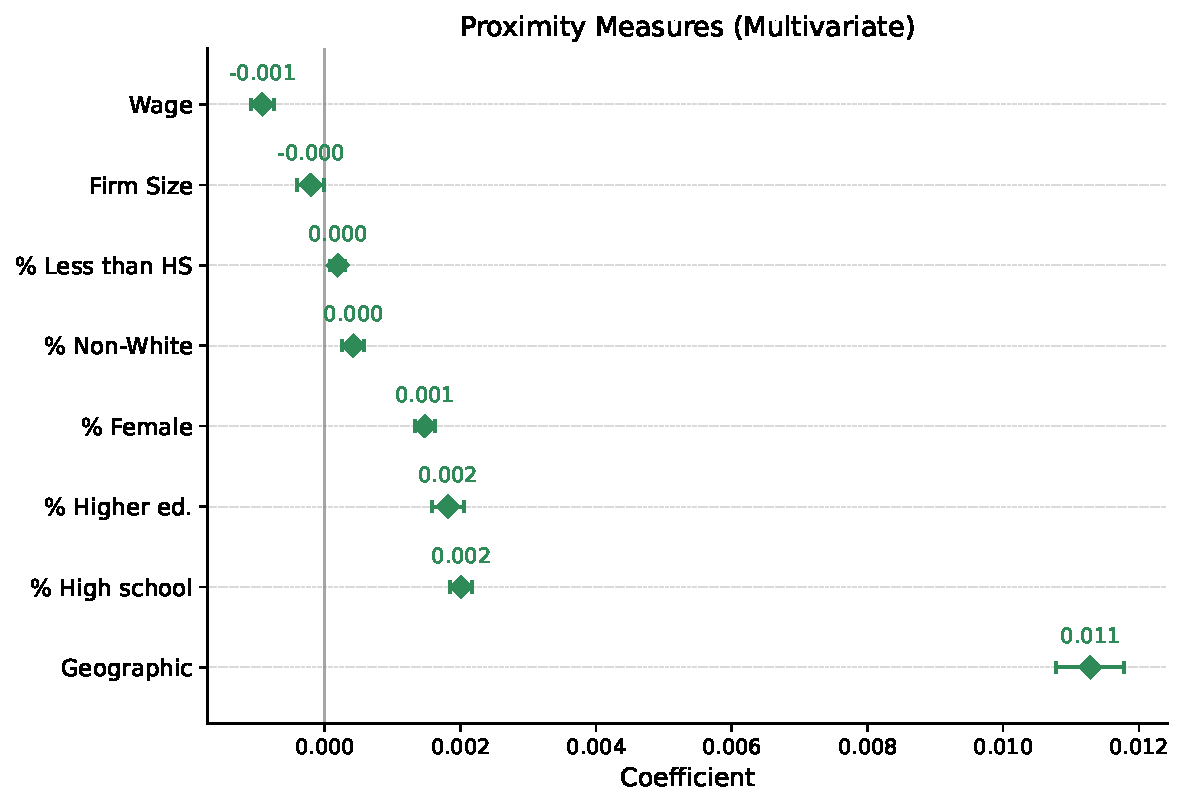
\includegraphics[width=\textwidth]{coefplot_bilateral_proximity_multivariate.pdf}
    \caption{Proximity Measures}
    \label{fig:bilateral_proximity_multivariate}
\end{subfigure}
\begin{subfigure}{0.49\textwidth}
    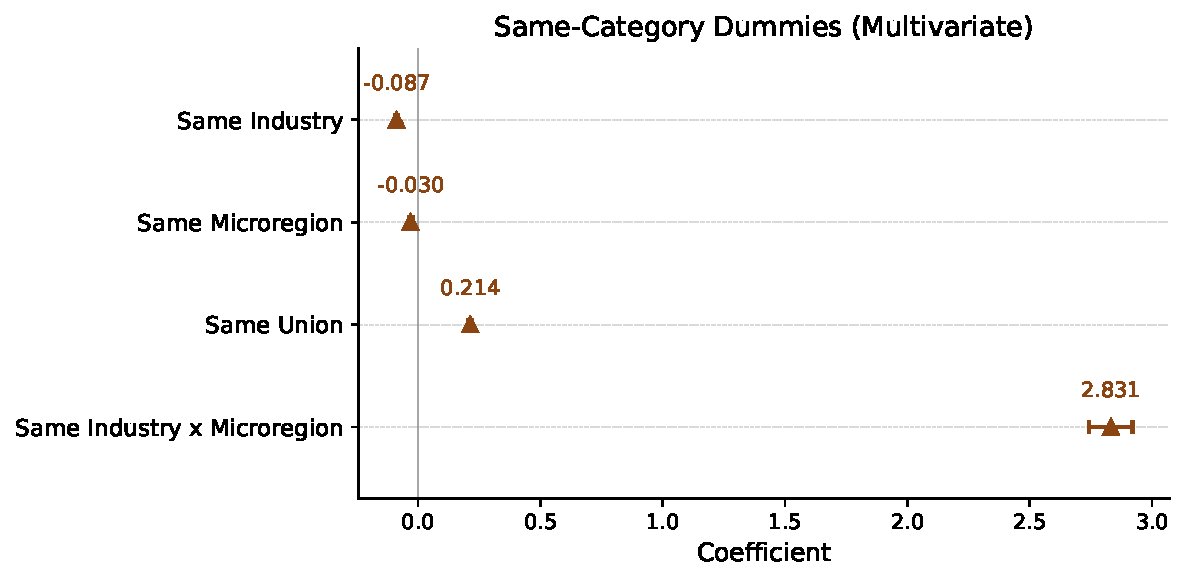
\includegraphics[width=\textwidth]{coefplot_bilateral_dummies_multivariate.pdf}
    \caption{Same-Category Dummies}
    \label{fig:bilateral_dummies_multivariate}
\end{subfigure}

\begin{tablenotes}
\footnotesize
\item \textit{Notes:} Coefficients from a single multivariate regression of post-treatment bilateral connectivity (2011--2015) on all predictors simultaneously, controlling for establishment $i$ fixed effects. Bilateral connectivity is measured as the person-weighted average flow of workers between establishment pairs across four consecutive year-pairs. Proximity measures are defined as the negative absolute difference between establishment characteristics (standardized), so higher values indicate greater similarity. Geographic proximity is measured as the negative log of distance between municipality centroids. Same-category dummies equal one if both establishments share the indicated category. Establishment characteristics are based on 2009--2011 pre-treatment averages. Horizontal lines represent 95\% confidence intervals based on robust standard errors. All regressions include the universe of establishment pairs, including those with zero worker flows.
\end{tablenotes}

\end{threeparttable}
\end{figure}
